\section{Software teori}
\textit{I dette afsnit beskrives den benyttede mikrokontroller (MCU) CY8CKIT-043 PSoC 4 M og dennes egenskaber. Dette gøres med henblik på at opnå forståelse for, hvordan denne kan benyttes til udvikling af systemet. Hertil beskrives MCUens centrale softwaremæssige funktioner samt digital signalkommunikation og -behandling.}

\subsection{CY8CKIT-043 Programmable System on Chip 4-M}
En mikrokontroller (MCU) er et elektrisk system, som kan kontrollere elektronisk udstyr ved hjælp af inkorporeret softwaredesign. En MCU er dermed en mindre computer, der forefindes i elektroniske enheder. Eksempelvis er MCUer at finde i fjernsyn, mobiltelefoner og printere. \citep{Scienceuddannelse,Tanenbaum2006} \newline
MCUer kan være bestående af en eller flere mikroprocessorer, hukommelse samt programmerbare in- og output-enheder. Dette giver brugeren af MCUen mulighed for at programmere enheden således, at denne kan kontrollere henholdsvis in- eller output-enheder. \citep{Scienceuddannelse,Tanenbaum2006} I dette projekt vil den tilgængelige MCU CY8CKIT-043 Programmable System on Chip (PSoC) 4 M-Series Prototyping Kit blive benyttet sammen med programmet PSoC Creator 3.3.

CY8CKIT-043 PSoC 4-M-Series Prototyping Kit er en MCU, som indeholder tre mikroprocessorer: to PSoCs og en Programmable Radio-on-Chip (PRoC), som alle ses på \figref{fig:PSoC}. \citep{CYPRESS2016PSoC}
\begin{figure}[H]
	\centering
	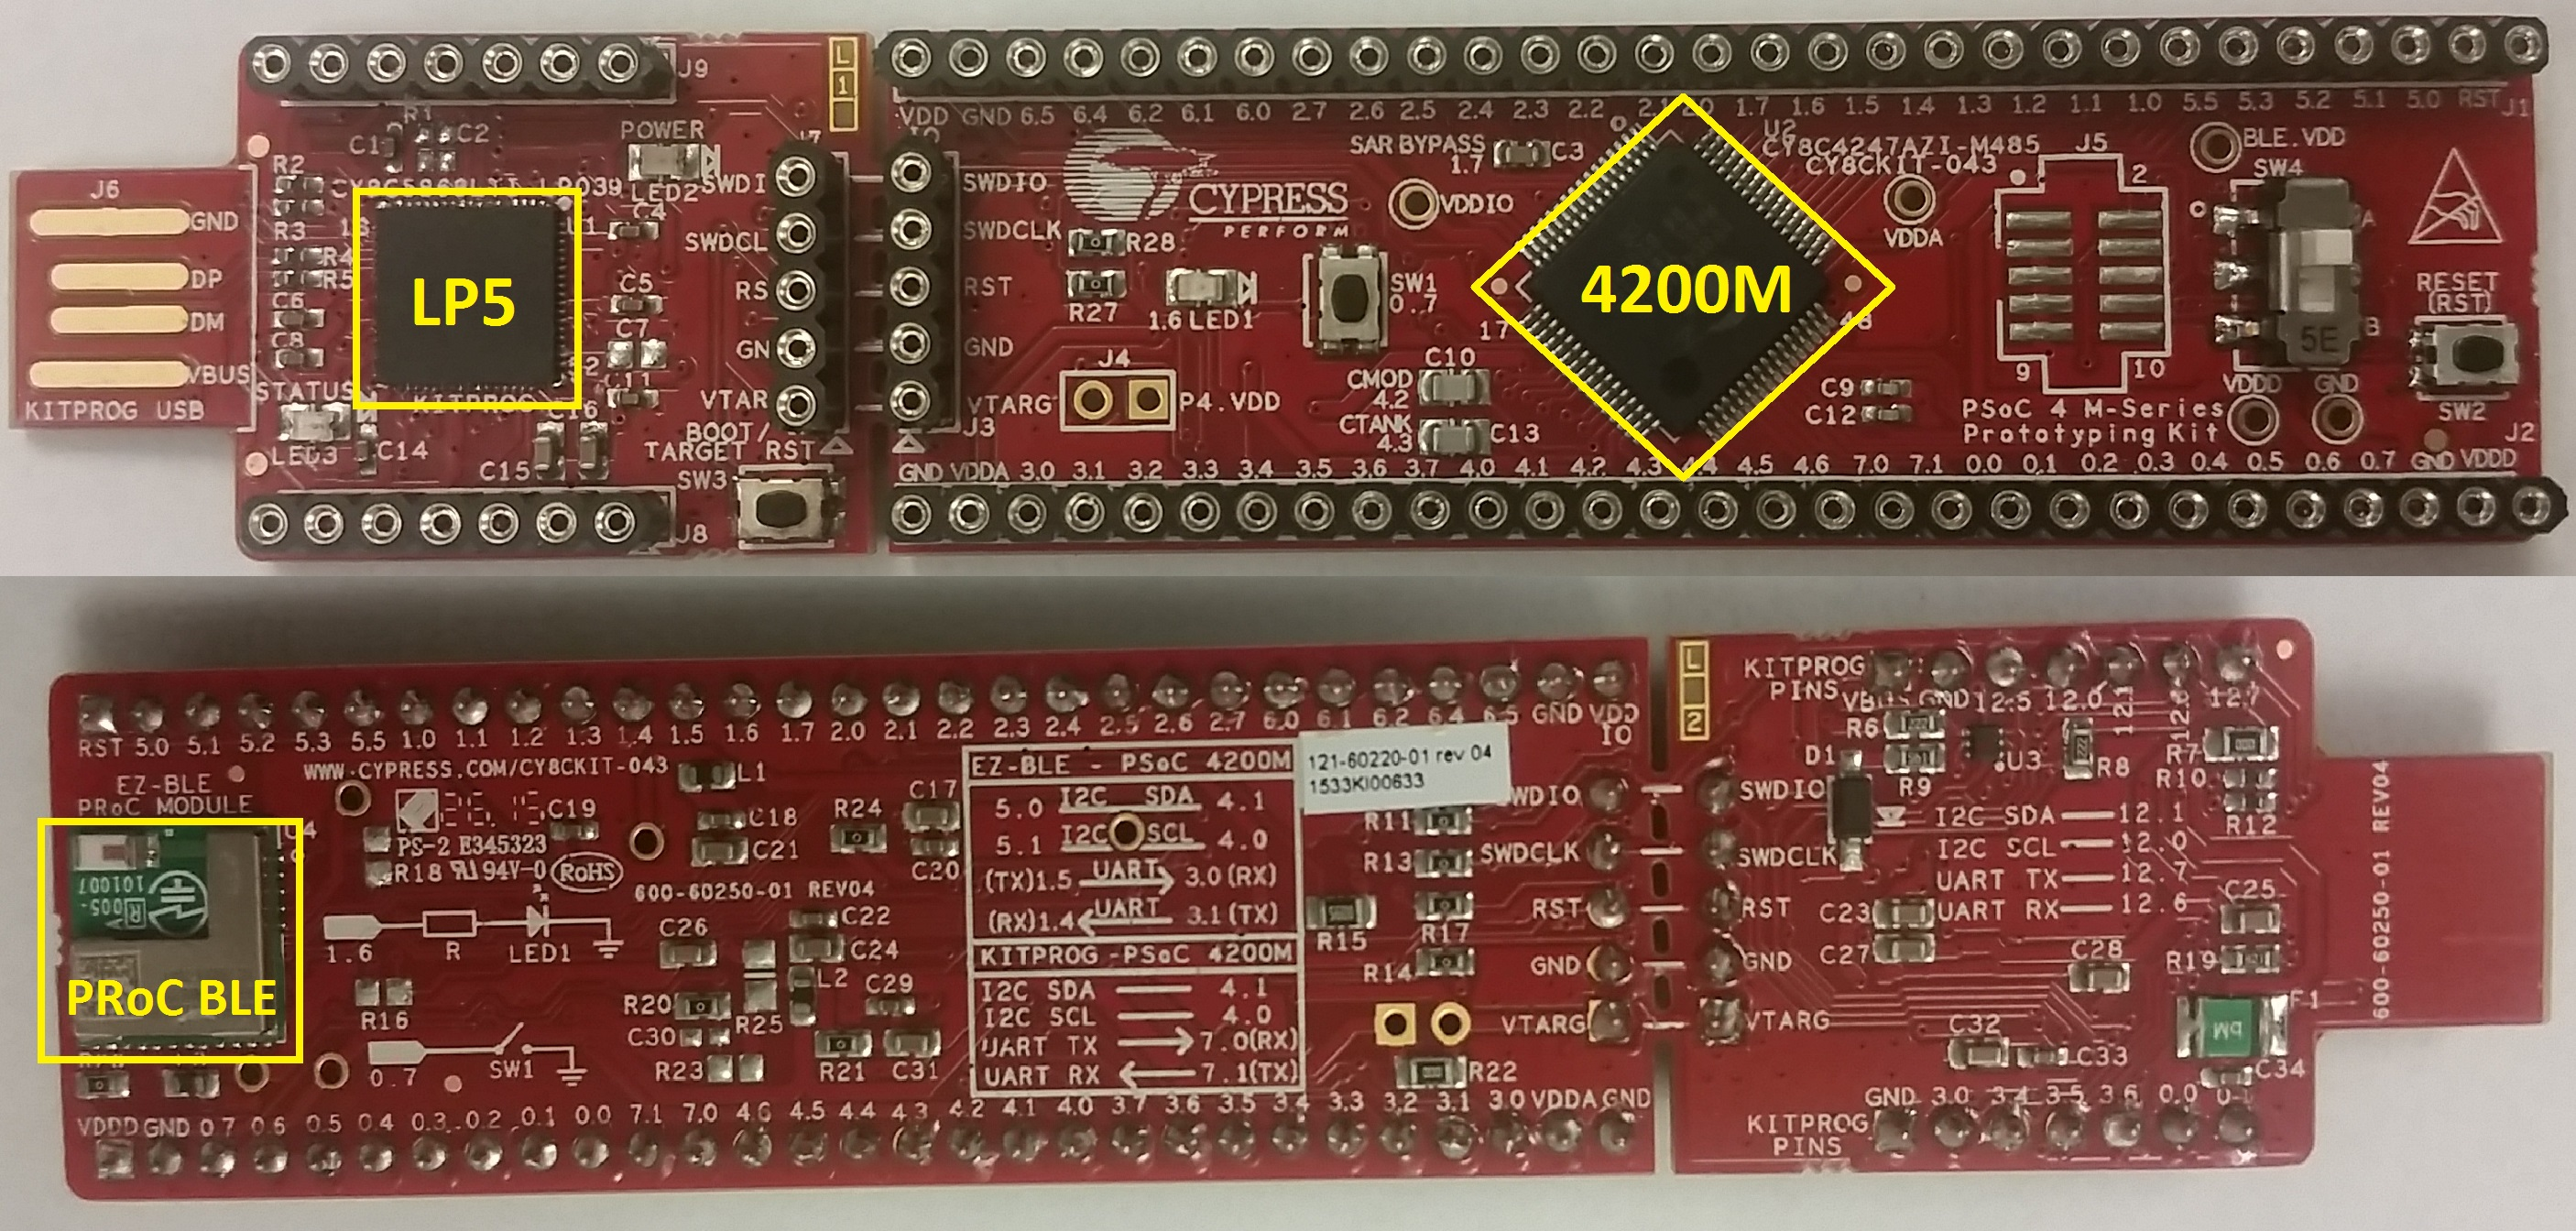
\includegraphics[scale=0.13]{figures/bProblemloesning/PSoC3.png}
	\caption{MCUen, CY8CKIT-043 PSoC 4 M-Series Prototyping Kit, er vist på dens forside og underside. MCUens LP5 og 4200M samt EZ\_BLE er markeret med gul. MCUen kan knækkes over i to til en KitProg board og target board del, hvilket er markeret med en gul streg på figuren. Kontakten til højre på forsiden af target boardet skal trykkes ned for, at PRoC programmeres på istedet for PSoC 4200M. Denne er ligeledes markedet med gul. \citep{CYPRESS2016PSoC,Semiconductor2016}}
	\label{fig:PSoC}
\end{figure}\vspace{-0.2cm}
Den første PSoC af typen LP5 sidder på MCUens KitProg board del, som er den del af MCUen, hvor universal serial bus (USB) porten er placeret. LP5 indeholder software, der kan indlæses på en computer ved hjælp af USB porten. Den bruges til at programmere og debugge softwaren på target boardet af MCUen, hvor PSoC 4200M er placeret. Denne mikroprocessor fungerer som hovedcomputeren og kodes til at bestemme, hvad target boardet skal foretage. På undersiden af target board delen er en PRoC med BLE placeret. Denne PRoC har ikke samme antal muligheder for afbenyttelse i forhold til PSoC 4200M. Dette skyldes, at BLE kræver meget plads og ydeevne for at være funktionel, hvorfor dets resterende ydeevne er begrænset.~\citep{CYPRESS2016PSoC,Semiconductor2016,CYPRESS2016Cortexm0}

For at opsamle data benyttes to MCUer, hvoraf den ene fungerer som master og den anden som slave. Masteren er tilkoblet en computer gennem USB samtidig med, at slaven er placeret på det objekt, som data skal opsamles fra. Dataoverførslen mellem disse enheder foregår gennem brug af BLE. I dette tilfælde benyttes en MCU fra Cypress, hvormed masterenheden og slaveenheden omtales som henholdsvis generic access profile (GAP) central og GAP peripheral \citep{Luthra2015}.

Generel kommunikationen mellem en master og en slave i et integreret system udføres ved brug af enten Serial Peripheral Interface (SPI) eller Inter-Integrated Circuit (I$^{2}$C) interface. Disse interfaces er kommunikationsprotokoller, som benyttes internt i eksempelvis MCUer til kommunikation mellem mikroprocessorer. Der findes derfor serielle porte med to ledninger til at sende data (TX) og modtage data (RX) imellem mikroprocessorerne på MCUen. \citep{Semiconductor2016} \newline
SPI er en kommunikationsprotokol, som blandt andet benyttes til full-duplex kommunikation, hvilket giver mulighed for både at sende og modtage data. En SPI bus involverer én master og en eller flere slaver. SPI busser benytter derfor fire ledninger til at skabe forbindelser mellem én master og én slave. I tilfælde af, at der er benyttes flere slaver til én master kræves det, at alle slaver har hver sin chip select. SPI er en hurtig kommunikationsprotokol på trods af pladskrævende elementer, når et større antal slaver tilkobles. \citep{Semiconductor2016,Sparkfun2016} \newline
Yderligere findes I$^{2}$C, som ligeledes er en computerbus dataprotokol. Masteren i systemet kontrollerer I$^{2}$C bussen og sender kommandoer til slaven. Både masteren og slaven kan sende og modtage data, men masteren kontrollerer, hvornår dette kan finde sted. I$^{2}$C kan, modsat SPI, involvere flere mastere til kommunikation med et givent antal slaver. Ydermere er I$^{2}$C en mere kompleks kommunikationsprotokol men samtidig mindre ressourcekrævende end SPI. Dette skyldes, at I$^{2}$C blot kræver to ledninger til at skabe forbindelse mellem master og slave.~\citep{Semiconductor2016,Sparkfun2016} %En MCU kræver en ekstern strømkilde for at kunne fungere. Ved forbindelse med en USB port adapteres spændingsforsyningen til 5V, men det er yderligere muligt at tilkoble en spænding til MCUens lav-volt applikation, hvilket gør den trådløs. \newline %Den benyttede MCU påkræver en spændingstilkobling i området 1,71~V til 5,50~V, når MCUen ikke er tilkoblet en USB port. Dermed skal VDD tilsluttes dette spændingsinterval fra en reguleret spændingsforsyning, for at overholde MCUens arbejdsområde. \citep{Semiconductor2016,Semiconductor20164200M}

Programmet PSoC Creator benyttes til at designe hardware og software til MCUen.\fxnote{Den kan designe hardwaren, fordi man trækker analoge blokke ind i hardware designet. Inden man bruger en pin på MCUen er denne låst, med mindre man definerer brugen af denne pin inde i topdesignet} Dette program benyttes til at designe og kode MCUen, hvorved softwaren kan tilpasses de fysiske komponenter i C kodning. \citep{Semiconductor2016} Når MCUen er tilsluttet computeren og sender data via Universal Asynchronous Receiver Transmitter (UART), kan MATLAB fungere som en GUI. Dette muliggør realtime visualisering af den data, som eksempelvis GAP central modtager fra GAP peripheral. \citep{Semiconductor2016,Sparkfun2016}

\subsection{Mikrokontrollerens target processor}
Mikroprocessoren 4200M er target processoren på CY8CKIT-043 PSoC 4 M-Series Prototyping Kit. Denne mikroprocessors kodning foretages i PSoC Creator og er dermed indeholdende de instruktionerne, som skal eksekveres, når MCUen er funktionel. Mikroprocessoren 4200M besidder ydermere en ARM Cortex-M0 processer. \newline
Mikroprocessoren er basseret på Instruction Set Architecture (ISA). ISA er bindeleddet mellem MCUens hardware og software. C kodning af softwaren muliggør dermed, at instruktioner kan blive udført i forbindelse med MCUens hardware. ISAs kategorier kan blandt andet være Reduced Instruction Set Computer (RISC) eller Complex Instrucion Set Computer (CISC). \citep{CYPRESS2016Cortexm0,Semiconductor20164200M,Yadav2016} \newline
Den benyttede MCUs mikroprocessor 4200M er af kategorien RISC. Denne processormetode benytter simple instruktioner, som kan blive eksekveret under én clock cycle. Derimod kræver dette mere Random Access Memory (RAM) kapacitet, da hver opgave hentes ned, processeres over flere omgange og gemmes indtil de er eksekveret. Denne metode tillader dog pipelinning, hvilket gør at flere instruktioner kan køre samtidig. En CISC baseret computer vil derimod udføre opgaver med så få linjer som muligt. Processorens hardware vil dermed være opbygget til at forstå og udføre komplekse instruktioner, hvilket kræver flere transistorer end RISC metoden.\fxnote{fetch - decode - exicute. Mere laves samtidig} Sammenligneligt er RISC processen hurtigere end CISC, men CISC computere kan udføre flere komplekse instruktioner på færre linjer end RISC. \citep{CYPRESS2016Cortexm0,Semiconductor20164200M,Yadav2016}\\
CPUen i Cortex-M0 er en del af det 32-bit MCU delsystem, som optimerer energibesparende drift ved hjælp af clock gating\fxnote{Clock gating saves power by adding more logic to a circuit to prune the clock tree. Pruning the clock disables portions of the circuitry so that the flip-flops in them do not have to switch states. Switching states consumes power. When not being switched, the switching power consumption goes to zero, and only leakage currents are incurred}. CPUen har en flash hukommelse på 128~kB og 16~kB RAM af typen SRAM. Algoritmen for MCUen gemmes i flash hukommelsen, da RAM hukommelsen kræver konstant spændingstilførsel og slettes, hvis spændingstilførslen til MCUen slukkes. \citep{Semiconductor20164200M}

\subsection{Power modes for mikrokontrolleren}
CY8CKIT-043 PSoC 4-M moduler besidder fem forskellige power modes: active, sleep, deep-sleep, hibernate og stop. Strømforbruget, samt tiden det tager at vågne op fra tilstandene, ses i \tabref{tab:Powermode} for PSoC 4200M. \citep{Semiconductor2016PowerMode}
\begin{table}[H]
	\centering
	\begin{tabular}{lcc} \hline
		\rowcolor[HTML]{C0C0C0} 
		Power mode & Strømområde &  \begin{tabular}[c]{@{}c@{}}Opvågningstid\\ for PSoC 4200M \end{tabular} \\ \hline
		Active & 1,3~mA til 14~mA & - \\ \hline
		Sleep & 1,0~mA til 3~mA & 0 \\ \hline
		Deep-sleep & 1,3~$\mu$A til 15~$\mu$A & 25~$\mu$s \\ \hline
		Hibernate & 150~nA til 1~$\mu$A & 0,7~ms \\ \hline
		Stop & 20~nA til 80~nA & 2~ms \\ \hline
	\end{tabular}%
	\caption{I tabellen ses strømforbruget samt opvågningstiden ved givne power modes for PSoC 4200M. \citep{Semiconductor2016PowerMode} (Modificeret)}
	\label{tab:Powermode}
\end{table}\vspace{-0.2cm}
Mikroprocessorens strømforbrug afhænger yderligere af, hvor meget af indholdet i mikroprocessoren der gøres utilgængeligt, hvilket illustreres i \tabref{tab:aktiv_inaktiv_CPU}. Det kan derfor være fordelagtigt at køre i en lav strømforbrugende tilstand, hvis der benyttes et batteri til at forsyne MCUen. En oversigt over MCUens funktionaliteter under de forskellige power modes ses i \tabref{tab:aktiv_inaktiv_CPU}. \citep{Semiconductor2016PowerMode}
\begin{table}[H]
	\centering
	\resizebox{\textwidth}{!}{%
	\begin{tabular}{lccccc} \hline
		\rowcolor[HTML]{C0C0C0} 
		Subsystem & Active & Sleep & Deep-sleep & Hibernate & Stop \\ \hline
		CPU & Aktiv & Tilbageholdt & Tilbageholdt & Deaktiveret & Deaktiveret \\ \hline
		RAM &  Aktiv &  Aktiv & Tilbageholdt & Tilbageholdt & Deaktiveret \\ \hline
		I$^{2}$C slave & Aktiv &  Aktiv &  Aktiv & Deaktiveret & Deaktiveret \\ \hline
		Høj-hastigheds clock & Aktiv & Aktiv & Deaktiveret & Deaktiveret & Deaktiveret \\ \hline
		ADC &  Aktiv &  Aktiv & Deaktiveret & Deaktiveret & Deaktiveret \\ \hline
		\begin{tabular}[l]{@{}l@{}}Low-power\\ komparatorer \end{tabular}&  Aktiv &  Aktiv &  Aktiv &  Aktiv & Deaktiveret \\ \hline
		\begin{tabular}[l]{@{}l@{}}	Generel-purpose \\ input/output (GPIO)\end{tabular} &  Aktiv &  Aktiv &  Aktiv &  Aktiv & Frosset \\ \hline
	\end{tabular}%
	}
	\caption{I tabellen ses hvilke subsystemer, der er henholdsvis aktive, tilbageholdte, deaktiverede eller frosset under de fem forskellige power modes. Hvis en funktion tilbageholdes, fungerer dens centrale konfiguration ikke, men alle eksterne funktioner er aktive. Når GPIO er frosset, er alle pins låst og kan derfor ikke modtage input- eller sende outputinformation. (Modificeret) \citep{Semiconductor2016PowerMode}}
	\label{tab:aktiv_inaktiv_CPU}
\end{table}\vspace{-0.25cm}
I sleep mode tilbageholdes CPUen, hvilket betyder at den venter på ethvert interrupt eller manuel genstart for at vågne op. RAMen bevares, men CPUen skriver eller læser ikke fra den, hvorfor CPUen ikke kører instruktionerne.\fxnote{Den sover ikke helt eller er ikke helt inaktiv - man kan sige, at den sover meget let, for den er til dels inaktiv, men den vækkes meget let.} Denne tilstand er fordelagtig til at reducere strømforbruget mellem hændelser som eksempelvis AD-konvertering. \citep{Semiconductor2016PowerMode} \\
Under deep-sleep er højfrekvente clocks deaktiveret, og da ADCen kræver sådanne clocks, er den ligeledes inaktiv under tilstanden. Deep-sleep mode kan benyttes, hvis høj ydeevne i analoge eller digitale enheder ikke kræves for funktionen. Tilstanden deep-sleep kræver specifikke interrupts for at vågne, som eksempelvis et I$^{2}$C eller GPIO interrup. Disse operationssystemer er aktive og fortsat fungerende som slave, hvormed de kan skabe et interrupt. \citep{Semiconductor2016PowerMode} \\
Når mikroprocessoren er i hibernate mode, er alle clocks og eksterne enheder deaktiveret. RAMen gemmes, men når et specifikt interrupt vækker mikroprocessoren, nulstilles og genstartes hele enheden. Denne tilstand kan vælges, hvis der kun er behov for periodiske opvågninger, og enheden skal bruge under 1~$\mu$A strøm. \citep{Semiconductor2016PowerMode} \\
Stop mode er den mindst strømforbrugende tilstand. Her modtager mikroprocessoren strøm, som bevarer logiske tilstande, mens alt andet er deaktiveret. Kun én dedikeret pin kan vække enheden fra denne stop mode, hvorefter den nulstilles og genstarter. Stop mode kan benyttes, når enheden ikke skal slukkes helt men skal være i stand til at tænde eksempelvis ved en trykknap med input i den dedikerede pin. \citep{Semiconductor2016PowerMode}

\subsection{Universal Asynchronous Receiver Transmitter}
En UART er en enhed, der implementerer seriel data og er dermed et led mellem et parallelt og et serielt interface, der både modtager og sender data. Data sendes som bits og kan både sendes serielt eller parallelt. \citep{Jimb02016a,Chun-zhiYin-shuiLun-yao2011} Parallelt bliver flere bits overført på samme tid, hvormed et 8-bit system er nødsaget til at have otte ledninger, hvor der i den ene ende er en RX kobling og i den anden er en TX kobling. \citep{Jimb02016a} Den serielle kommunikation foregår asynkront og kan foregå med én ledning, da kun en bit overføres af gangen. Den serielle kommunikation benyttes oftest, da der ikke kræves så mange ledninger. Det er i den serielle kommunikation nødvendigt at bestemme en baudrate\fxnote{baudrate = Hvor hurtigt der sendes data (bits per sekund[bps])}, som TX og RX synkroniseres efter. Det modtagne data gemmes ofte i en buffer, som efterfølgende videregives i form af first-in-first-out (FIFO). \citep{Jimb02016a}\newline 
Overførsel af data sker asynkront, som det ses på \figref{fig:asynkron}.
\begin{figure}[H]
	\centering
	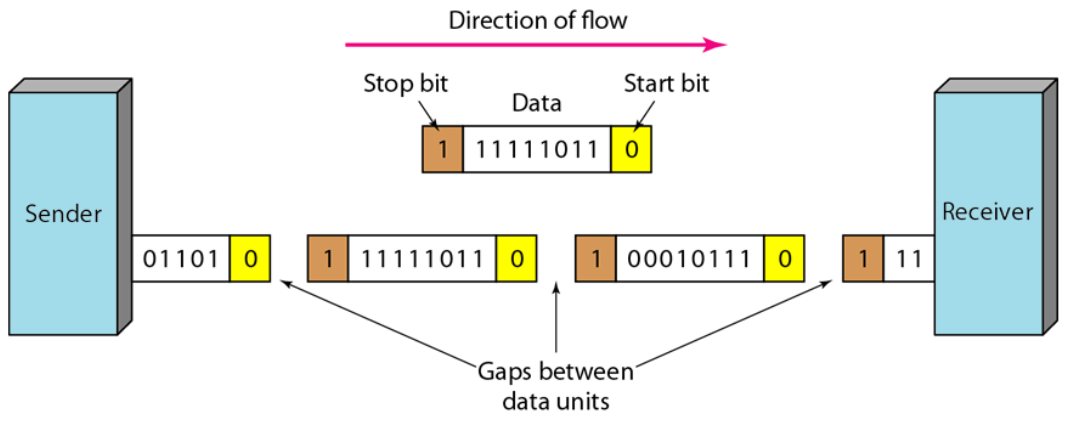
\includegraphics[scale=0.5]{figures/bProblemloesning/asynkron.png}
	\caption{På figuren ses en asynkron dataoverførsel mellem en afsender TX og en modtager RX. Dataenhederne sendes ved brug af et start- og stopbit for alle afsendte enheder. \citep{Jimb02016} (Modificeret)}
	\label{fig:asynkron}
\end{figure}\vspace{-0.25cm}
Ved denne kommunikationsform opererer RX og TX ved to forskellige clocks. For at opnå synkront data sættes et startbit og stopbit\fxnote{alt udenfor disse overføres ikke}, hvilket illustreres på \figref{fig:asynkron}. Data i gaps mellem stop- og startbit kasseres. UARTens opgave er at læse parallel data fra FIFO, som laves om til seriel data. Dette data kan efterfølgende sendes til andre enheder. Når RX i en anden enhed modtager et startbit, laves data om fra seriel til parallel data, hvorefter data kan skrives til modtager-FIFO. \citep{Jimb02016a,Chun-zhiYin-shuiLun-yao2011}

Nogle enheder indeholder mere end én seriel-linje, og disse enheder fungerer enten som fuld-duplex eller halv-duplex. Fuld-duplex enheder kan både sende og modtage data på samme tid. Halv-duplex enheder sender og modtager data på skift. \citep{Jimb02016a,Chun-zhiYin-shuiLun-yao2011}

\subsection{Interrupts}
Interrupt er en funktion, som kan afbryde Central Processing Unit (CPU) fra main filen ved at løfte et ben højt ved en bestemt hændelse, eller hvis en timer har talt op til et bestemt niveau. \citep{Badiger2016} \\
I en aktivitetsmåler kan interrupts blandt andet benyttes til at vække gyroskopet fra sleep mode til detektion af cykling. Hvis denne aktivitetsform ikke finder sted, lægges benet for funktionen ned igen og aktivitetsmåleren fortsætter som ellers ved at behandle accelerometer data.

En CY8CKIT-043 PSoC 4-M besidder 32 interrupt linjer (IRQ), IRQ[0] til og med IRQ[31], som kan prioriteres efter fire niveauer. Når et interrupt finder sted, vil CPUen modtage en specifik funktion, som kaldes Interrupt Service Routine (ISR). Denne skal sørge for, at koden til interrupt eksekveres hurtigst muligt, hvorved mainprogrammet ikke afbrydes konstant. Koden til interrupt bliver eksekveret, hvorefter main filen fortsættes. \citep{Badiger2016}\\
Inden et interrupt er programmet i tread mode, hvilket ses på \figref{fig:interrupt}. Når et interrupt finder sted, vil en pin gå høj, og processoren overfører information til den nuværende stack. Dette kaldes for stacking, hvilket får main filen til at gå i handler mode. Her skifter pointeren også stilling fra Main Stack Pointer (MSP) til Process Stack Pointer (PSP). Dette betyder, at den pågældende funktion gemmes og sættes på pause. Det er derved muligt at vende tilbage til præcis samme sted i processen efter interruptet. Koden for ISR eksekveres, hvorefter pinen lægges ned igen og unstacking foregår. Main filen går igen i tread mode, pointeren skifter til MSP og hovedarbejdet fortsættes. \citep{Tanenbaum2006,Badiger2016}
\begin{figure}[H]
	\centering
	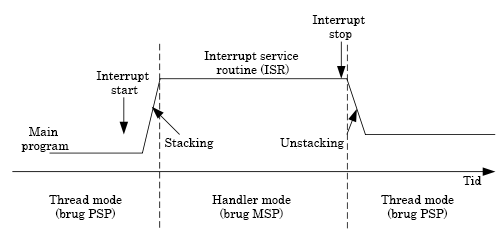
\includegraphics[scale=0.68]{figures/bProblemloesning/interrupt.png}
	\caption{På figuren ses effekten af et interrupt. Det fremgår, at et interrupt afbryder CPUens main rutine, for dermed at eksekvere den kode som er tilhørende ISR. Når ISR er udført vender CPUen tilbage til eksekveringen af main rutinen. \citep{Tanenbaum2006}}
	\label{fig:interrupt}
\end{figure}\vspace{-0.5cm}
I en Advanced RISC Machines (ARM) Cortex-M0 kan en høj prioritet afbryde en lav prioritet. Hver gang et interrupt finder sted, er der risiko for et stack overflow. Dette hænder, hvis afbrydelserne fortsætter i uendelighed, og det ikke er muligt af finde ud af, hvor i prosessen interruptet skal vende tilbage til. Igennem unstacking genskabes registrene, hvor afbrydelsen oprindeligt fandt sted. \citep{Badiger2016}

Der findes forskellige slags interrupts, som blandt andet kan finde sted på grund af manuel udløsning eller algoritmer. Næsten alle interrupts er programmerbare i CY8CKIT-043 PSoC 4-M. Der findes dog fem interrupts, som ikke kan ignoreres og kaldes exceptions. Disse er prioriteret højere end alle andre interrupts, da de beskytter og sikre mod fejl. \fxnote{Watch Dog timeren genstarter og har aller højest prioritet af alle interrupts}\fxnote{http://flint.cs.yale.edu/cs422/doc/art-of-asm/pdf/CH17.PDF (Sidetal 1000)}\citep{Badiger2016}

\subsection{Clocks}
Clocks er et kredsløb, som benyttes til at synkronisere for eksempel rækkefølgen af funktioner eller indstilling af to signaler, hvormed en clock kontrollerer tiden for et program. En clock udsender ved hjælp af oscillatorer en række impulser, der skifter mellem værdierne 0 og 1 med præcis pulsbredde og interval. Tidsintervallet imellem henholdsvis to pulsers stigning fra 0 til 1 eller fald fra 1 til 0 kaldes clock cycle time, og pulsfrekvensen indstilles herefter. Pulsfrekvensen kontrolleres ofte af en crystal oscillator, da dette gør frekvensen mere præcis. \citep{Tanenbaum2006}

En clock er et helt grundlæggende element i MCUer. Den kan eksempelvis bruges til at lave interrupts i et bestemt tidsinterval, hvis der er behov for, at en funktion skal køres igennem på bestemte tidspunkter\fxnote{Når gyroskopet skal vækkes op hvert tiende skund}. Derudover kan en clock eksempelvis benyttes som måleenhed for funktioners varighed. Derved opnås bevidsthed om, hvornår to funktioner skal påbegyndes, hvis de har forskellige clock cykles men skal være afsluttet samtidig. \citep{Tanenbaum2006}

Clock systemet for PSoC 4200M består af en Watch Crystal Oscillator (WCO), der kører med 32 kHz. Derudover findes en Internal Main Oscillator (IMO), som per standardindstilling kører med 24 MHz men kan fungere fra 3 til 48 MHz, og en Internal Low-speed Oscillator (ILO), der normalt kører med 32 kHz. IMO er den primære kilde til intern clocking i PSoC 4200M ved aktiv tilstand, hvorimod ILO kan generere clocks under deep sleep mode. WCO kan både benyttes under aktiv og deep-sleep mode. Denne oscillator kan desuden benyttes som en real-time clock, hvilket holder styr på den aktuelle tid.\fxnote{Når vi ved, om vi skal bruge clocks, og i så fald hvilke, kan disse eventuelt blive beskrevet her.} \citep{Semiconductor20164200M}
%http://www.hardwaresecrets.com/how-a-cpu-works/2/

\subsection{Analog-til-digital konverter}
En ADC benyttes, når analogt data skal konverteres til digitalt data, således det kan bearbejdes eller visualiseres af en digital enhed. Samplingsfrekvensen og opløsningen for en ADC er afgørende for, hvor repræsentativt det analoge signal bliver gengivet i den digitaliserede udgave. Ifølge Nyquists teori skal samplingsfrekvensen være mindst det dobbelte af den højeste frekvens i signalet for at sikre en repræsentativ gengivelse af det analoge signal og dermed undgå aliasing. \citep{Webster2011} \\
Der findes flere forskellige typer ADC, som for eksempel digital ramp ADC, sigma delta ADC og successive approximation (SAR) ADC. En digital ramp ADC tæller op fra 0 V for at finde det rette niveau for inputspændingen fra signalet. Når den rammer signalets spænding, overføres denne værdi til et digitalt output, referencespændingen nulstilles og tæller forfra igen. En sigma delta ADC oversampler og besidder kun en 1 bits konverter. Den foretager en sammenligning af en referenceværdi med inputspændingen, som enten giver 0 eller 1 som output. Disse værdier indsendes til et digitalt filter, der indsætter antallet af digitale ettaller og derved konverterer til et digitalt signal. Forskellen herimellem er altså metoden for konverteringen.~\citep{Moore2004,Sheingold2014} \\
I en SAR ADC, som er implementeret i MCUen CY8CKIT-043 PSoC 4-M, kommer signalet ind i en komparator, der har en referencespænding (Vref). Først sammenlignes inputsignalet (Vin) med Vref, som indstilles til at være halvdelen af arbejdsområdet. Komparatoren vurderer, om signalet er større eller mindre end denne værdi. Herved findes det mest betydende tal, hvorefter processen med halvering af Vref, som lægges til eller trækkes fra, og vurdering herudfra fortsætter indtil 12 bits er fundet. Derved er den analoge data konverteret til binære tal. Hvis en SAR ADC har for mange bits, bliver disse inddelingstrin så små, at det kan være støj, som afgør bitniveauerne. \citep{Moore2004,Sheingold2014} \\
Et eksempel på en SAR ADCs virkemåde ses på \figref{fig:SAR_ADC}
\begin{figure}[H]
	\centering
	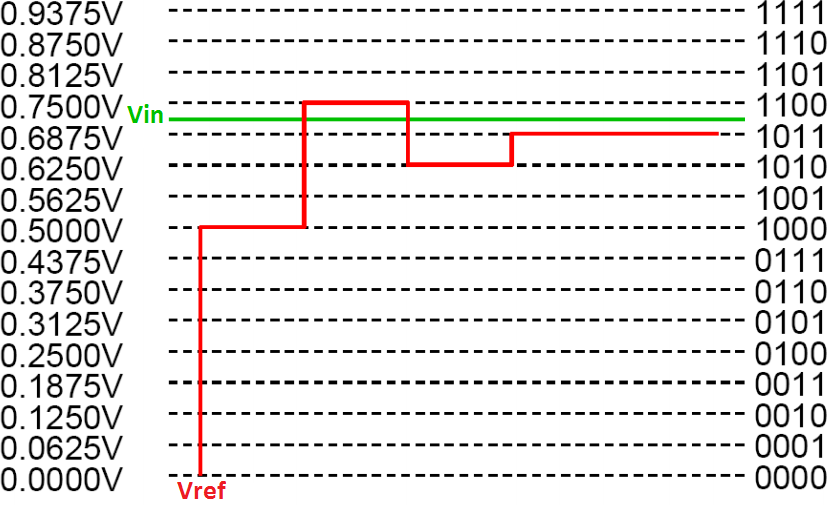
\includegraphics[scale=0.52]{figures/bProblemloesning/SAR_ADC.png}
	\caption{På figuren ses funktionen for en 4 bits SAR ADC. Vin er i dette tilfælde en konstant værdi men kan skifte værdi flere gange i sekundet.}
	\label{fig:SAR_ADC}
\end{figure}\vspace{-0.5cm}
På \figref{fig:SAR_ADC} ses det, at Vref indstilles til halvdelen af arbejdsområdet på 1~V, hvoraf komparatoren vurderer hvorvidt inputsignalet er større end Vref. Derefter adderes en fjerdel af arbejdsområdet til Vref og komparatoren foretager samme vurderingen. Denne proces fortsættes til alle bits er fundet, hvorefter det analoge signal er konverteret til et digitalt.

MCUens 12 bits SAR ADC kan inddele det analoge signal i 4096\fxnote{$2^12$} spændingsniveauer. Den skal derudover bruge 18 clocks for at fuldføre en 12 bits konvertering af data med samplingsfrekvens på 18.000.000 Hz, hvilket er dens maksimale samplingsfrekvens. MCUen kan indstilles til forskellige powermodes, hovraf ADCen eksempelvis ikke kan benyttes under deep-sleep\fxnote{da en klokfrekvens på 18MHz kræves, og denne hurtige clock er slukket under deep-sleep}. \newline 
ADCen understøtter både single ended og differential inputs og kan scanne alle 16 kanaler automatisk. Enhver ledig pin på MCUen kan monitoreres af ADCen. Det er muligt at have flere kanaler på ADCen, hvorved der kan samples ved forskellige frekvenser alt efter signalernes udformning. \citep{Semiconductor20164200M}

\subsection{Trådløs kommunikation via Bluetooth Low Energy} 
Bluetooth er en radiobølge teknologi, som er designet til trådløs kommunikation mellem elektroniske enheder. Der findes Bluetooth Smart enheder, som kun understøtter BLE, og Bluetooth Smart Ready enheder, der understøtter både klassisk Bluetooth og BLE. \citep{Sauter2011,Gupta2013}\\
Bluetooth er fordelagtigt at benytte, hvis der ønskes trådløs kommunikation eller trådløse enheder. PRoCens CPU på CY8CKIT-043 PSoC 4 M-Series Prototyping Kit er et EZ\_BLE PRoC modul, som besidder en ARM Cortex-M0 processer. Denne CPU har en 2,4 GHz BLE radio, som understøtter en datahastighed på 1 megabits per sekund (Mbps). Data videresendes med en chip antenne, der kan transmittere data ved en radiofrekvens mellem 2,4-2,5 GHz.~\citep{Semiconductor2016PRoC,Semiconductor2016BLEdyb}\\
Bluetooth sender og modtager radiobølger i bånd af 79 forskellige frekvenser, som kaldes kanaler. Bølgerne bliver modificeret af enheden, således de opfattes som et signal. Enheden, som skaber forbindelsen, vil automatisk være masteren og kan for eksempel kontrollere afsendelsen af data fra slaven samt styre varigheden af forbindelsen. Master og slave rollen kan dog skifte undervejs. Tilsammen vælger masteren og slaven en tilfældig kanal, men for at mindske risikoen for interferens skifter enhederne kanal op til tusinde gange i sekundet.~\citep{CYPRESS2016workshopBLE,Sauter2011} \\
BLE er en videreudvikling af Bluetooth og kaldes også Bluetooth version 4.0. BLE kræver mindre strøm for at fungere, fordi enheden er i sleep mode størstedelen af tiden. Når data sendes, aktiveres BLE og overfører hurtigst muligt, hvorefter den igen deaktiveres og går i deep sleep mode. Dette opnås ved, at BLE kun benytter 40 forskellige kanaler, hvor nogle kanaler er specielt dedikeret til at skabe forbindelse\fxnote{3 kanaler - klassisk bluetooth har 32} mellem enheder, og andre kanaler dedikeres til at sende data. Derved sikres en driftscyklus\fxnote{ratio mellem enheden er slukket og tændt} som er tæt på nul. Et BLE modul kan ikke skifte mellem master og slave rollen undervejs. Resultatet heraf medfører, at når en forbindelse er skabt, er rollerne fastlagt. Dette simplificerer designet yderligere, hvorved der ligeledes spares strøm. \citep{Gupta2013}